\documentclass[final,3p,times]{elsarticle}

\usepackage{amsmath,amssymb,amsthm,mathtools}
\usepackage{tikz}

\newtheorem{theorem}{Theorem}[section]
\newtheorem{proposition}[theorem]{Proposition}
\newtheorem{lemma}[theorem]{Lemma}
\newtheorem{corollary}[theorem]{Corollary}
\theoremstyle{definition}
\newtheorem{definition}[theorem]{Definition}

\newcommand{\PP}{\mathbb{P}}
\newcommand{\EE}{\mathbb{E}}
\newcommand{\TV}{d_{\mathrm{TV}}}
\newcommand{\HH}{d_{\mathrm{H}}}
\newcommand{\cO}{\mathcal{O}}
\newcommand{\BC}{\mathrm{BC}}
\newcommand{\one}{\mathbf{1}}

\begin{document}

\begin{frontmatter}

\title{Factorizations, symmetry reductions, and phase transitions in rowmotion Markov chains}

\author{Alexander Okezue Bell}
\address{Department of Mathematics, Stanford University, Stanford, CA, US}

\begin{abstract}
Rowmotion is a bijection on the distributive lattice $J(P)$ of order ideals of a finite poset $P$. The rowmotion Markov chain assigns probabilities $p_x$ to elements $x$, independently selects a random subset of maximal elements of the current ideal, and moves to the complement of the upset they generate. We develop factorization and symmetry-reduction tools and use them to analyze mixing and cutoff.

For Boolean lattices with inhomogeneous probabilities we prove an exact tensor-product decomposition into two-state chains. We show reversibility, compute an orthonormal eigenbasis and spectrum, and derive a closed formula for the chi-square distance from stationarity from any start. This yields matching constant-window total-variation bounds governed by a single moment function.

For disjoint unions we obtain an exact tensor-product factorization and show that $J(P)$ admits a nontrivial lattice product decomposition only when $P$ is disconnected. For $P=Q\sqcup A_m$ with fixed connected $Q$ and a large antichain $A_m$, symmetry yields a strong lumping to $J(Q)\times\{0,\dots,m\}$ with an explicit kernel, and cutoff transfers from the antichain factor. For tensor powers $Q^{\sqcup m}$ we lump to an occupancy chain of polynomial size and prove an exact Hellinger isometry, giving tensor-power cutoff profiles from one-copy Hellinger decay. We also compute orbit chains for symmetric connected families, highlighting two-sector metastability for complete bipartite orders and a top-rank cutoff transfer regime for ordinal sums of antichains.
\end{abstract}

\begin{keyword}
rowmotion \sep toggles \sep Markov \sep mixing \sep cutoff \sep lumping \sep posets
\end{keyword}

\end{frontmatter}

\section{Introduction}

Rowmotion is a cyclic action on the distributive lattice $J(P)$ of order ideals of a finite poset $P$.
It may be described either on ideals or on antichains, and it has appeared in the literature under several closely related names, including the Brouwer-Schrijver map \cite{BrouwerSchrijver1974}, the Fon-der-Flaass action \cite{FonDerFlaass1993}, the Panyushev complement in the setting of root posets \cite{Panyushev2009}, and rowmotion in dynamical algebraic combinatorics \cite{Striker2017Dynamical}.
Early work of Fon-der-Flaass and Cameron-Fon-der-Flaass established structural orbit properties and posed periodicity problems that have driven a large body of subsequent research \cite{FonDerFlaass1993,CameronFonDerFlaass1995}.
Rowmotion also sits in a broader landscape of cyclic actions on combinatorial objects, including Sch\"utzenberger promotion \cite{Schutzenberger1972Promotion} and its many variants.

A central organizing idea is locality.
Striker and Williams introduced the toggle group viewpoint and interpreted rowmotion and promotion as compositions of involutive local toggles \cite{StrikerWilliams2012}.
Thomas and Williams developed a slow motion description and structural generalizations, clarifying how local moves encode global dynamics \cite{ThomasWilliams2019Slow}.
These perspectives are part of dynamical algebraic combinatorics, which studies discrete dynamical systems on posets, tableaux, and related objects and emphasizes phenomena such as homomesy and resonance \cite{ProppRoby2015Homomesy,Striker2017Dynamical}.
Recent progress includes the proof of the Cameron-Fon-der-Flaass conjecture for plane partitions \cite{PatriasPechenik2020Dynamics}.
Birational lifts of rowmotion have also been developed and have revealed further structure \cite{MusikerRoby2019BirationalPaths}.

Defant, Li and Nestoridi introduced a randomized variant of rowmotion by inserting independent Bernoulli choices into the toggle description, producing a Markov chain on $J(P)$ called the rowmotion Markov chain \cite{DefantLiNestoridi2024Rowmotion}.
They proved a simple stationary distribution for a broad family of toggle Markov chains and established cutoff for Boolean lattices with a constant probability parameter \cite{DefantLiNestoridi2024Rowmotion}.
This line of work connects dynamical algebraic combinatorics to quantitative mixing, where cutoff for natural families of chains is a major theme \cite{Diaconis1996Cutoff}.
Product and tensor-power chains have a parallel cutoff theory that often uses Hellinger distance and related affinities \cite{ChenKumagai2018ProductCutoff}.

Rowmotion Markov chains inherit combinatorial symmetry from the underlying poset, while their state spaces can be extremely large.
This article develops two tools for analyzing mixing through that structure.
The first tool is exact factorization, which reduces a chain to a tensor product of smaller chains.
The second tool is exact symmetry reduction through strong lumpability, which compresses a chain along orbits of an automorphism group.
The interaction of these tools leads to explicit reduced chains, explicit distances to stationarity in some cases, and sharp predictions for the presence or absence of cutoff.
A representative reduced level graph for ordinal sums of antichains is shown in Figure~\ref{fig:level_chain}.

\subsection{Contributions}

For Boolean lattices with distinct probabilities on different coordinates, we show that the rowmotion chain is an exact tensor product of two-state chains, prove reversibility, compute an orthonormal eigenbasis and spectrum, and obtain a closed chi-square formula from any start state. From this we derive matching constant-window total variation bounds governed by a single moment function.

For disjoint unions of posets, we prove that the corresponding rowmotion chain is an exact tensor product. We also show that $J(P)$ admits a nontrivial lattice product decomposition if and only if $P$ is a disjoint union.

For $P=Q\sqcup A_m$ with fixed connected $Q$ and a large antichain $A_m$, the product structure and symmetry on $A_m$ yield a strong lumping to $J(Q)\times\{0,1,\dots,m\}$ with an explicit kernel, and cutoff transfers from the antichain factor. For $m$ identical components, permutation symmetry yields a strong lumping to an occupancy chain with polynomial state space size. This lumping preserves Hellinger distance exactly and yields tensor-power cutoff profiles governed by one-copy Hellinger decay.

For connected rank-transitive posets, we compute explicit orbit chains. Complete bipartite orders exhibit a metastable two-sector mechanism. Ordinal sums of antichains yield a low-dimensional orbit chain with closed-form level weights and transition rates and a phase transition separating top-rank cutoff transfer from metastable slowdown.

\subsection{Organization}

Section~2 reviews rowmotion Markov chains, mixing distances, and lumpability, including orbit lumping under group symmetry.
Section~3 treats Boolean lattices with inhomogeneous probabilities and gives an explicit diagonalization and sharp mixing bounds.
Section~4 develops factorization for disjoint unions, rigidity of lattice products, the large antichain factor family $Q\sqcup A_m$, and tensor-power occupancy reductions.
Section~5 treats rank-transitive connected families and derives reduced orbit chains and asymptotic mixing behavior.
Section~6 discusses open problems and future directions.

\section{Preliminaries}

\subsection{Posets, order ideals, and rowmotion Markov chains}

Let $P$ be a finite poset.
An order ideal is a subset $I\subseteq P$ such that $y\le x\in I$ implies $y\in I$.
Let $J(P)$ denote the set of order ideals.
For a subset $S\subseteq P$, let
\[
\uparrow S:=\{y\in P: \exists x\in S\text{ with }x\le y\}
\]
be the upset generated by $S$.
For an order ideal $I$, let $\max(I)$ be its set of maximal elements.

Fix probabilities $p_x\in(0,1)$ for all $x\in P$.
The rowmotion Markov chain $\mathbf{M}_{J(P)}$ is the chain on $J(P)$ defined as follows.
From state $I\in J(P)$, choose a random subset $S\subseteq \max(I)$ by including each $x\in \max(I)$ independently with probability $p_x$ and transition to the new state
\[
I' = P\setminus \uparrow S.
\]
This is the definition in \cite{DefantLiNestoridi2024Rowmotion}.

A main result of \cite{DefantLiNestoridi2024Rowmotion} gives the stationary distribution.

\begin{theorem}[Stationary distribution \cite{DefantLiNestoridi2024Rowmotion}]\label{thm:DLN_stationary}
Assume $\mathbf{M}_{J(P)}$ is irreducible and $p_x\in(0,1)$ for all $x\in P$.
Then the stationary distribution $\pi$ satisfies
\[
\pi(I)\ \propto\ \prod_{x\in I} p_x^{-1}.
\]
\end{theorem}

\subsection{Mixing distances}

For probability measures $\mu,\nu$ on a finite set $\Omega$, the total variation distance is
\[
\TV(\mu,\nu) = \frac12\sum_{\omega\in\Omega}|\mu(\omega)-\nu(\omega)|.
\]
For a Markov chain with stationary distribution $\pi$, the mixing time at level $\varepsilon\in(0,1)$ is
\[
t_{\mathrm{mix}}(\varepsilon) = \min\{t\ge 0: \sup_{x\in\Omega}\TV(\delta_x K^t,\pi)\le \varepsilon\}.
\]

We use Hellinger distance and the Bhattacharyya coefficient.
For probability measures $\mu,\nu$ on $\Omega$,
\[
\BC(\mu,\nu)=\sum_{\omega\in\Omega}\sqrt{\mu(\omega)\nu(\omega)},
\qquad
\HH(\mu,\nu)^2 = 2\bigl(1-\BC(\mu,\nu)\bigr).
\]
Standard inequalities compare total variation and Hellinger distance, see \cite[Chapter 4]{LevinPeresWilmer2017}.
For all $\mu,\nu$,
\begin{equation}\label{eq:TV-H}
\TV(\mu,\nu)\le \HH(\mu,\nu)\le \sqrt{2\,\TV(\mu,\nu)}.
\end{equation}

We also use chi-square divergence.
For $\mu$ absolutely continuous with respect to $\pi$,
\[
\chi^2(\mu\|\pi)=\sum_{\omega\in\Omega}\frac{(\mu(\omega)-\pi(\omega))^2}{\pi(\omega)}.
\]
Cauchy--Schwarz gives
\begin{equation}\label{eq:TV-chi2}
\TV(\mu,\pi)\le \frac12\sqrt{\chi^2(\mu\|\pi)}.
\end{equation}

\subsection{Strong lumpability and orbit lumping}

Let $K$ be a Markov kernel on a finite set $\Omega$.
A partition $\mathcal{A}=\{A_1,\dots,A_m\}$ of $\Omega$ is strongly lumpable if the block process is Markov for every initial distribution.
Kemeny and Snell gave a necessary and sufficient criterion.

\begin{theorem}[Lumpability criterion \cite{KemenySnell1960}]\label{thm:lumpability}
A partition $\mathcal{A}=\{A_1,\dots,A_m\}$ is strongly lumpable if and only if for all blocks $A_i,A_j$ and all $x,x'\in A_i$,
\[
\sum_{y\in A_j}K(x,y)=\sum_{y\in A_j}K(x',y).
\]
\end{theorem}

Orbit partitions of group actions provide a common source of lumpability.

\begin{theorem}[Orbit lumping]\label{thm:orbit_lumping}
Let a finite group $G$ act on $\Omega$ and let $K$ be a Markov kernel on $\Omega$.
Assume $K$ is $G$-equivariant, meaning $K(gx,gy)=K(x,y)$ for all $g\in G$ and $x,y\in\Omega$.
Then the partition of $\Omega$ into $G$-orbits is strongly lumpable.
\end{theorem}

\begin{proof}
Let $B$ be a $G$-orbit and let $x,x'\in B$.
Since $B$ is an orbit there exists $g\in G$ with $x'=gx$.
Then
\[
\sum_{y\in B}K(x',y)=\sum_{y\in B}K(gx,y)=\sum_{y\in B}K(x,g^{-1}y).
\]
Since $g^{-1}$ permutes $B$, the map $y\mapsto g^{-1}y$ is a bijection on $B$, so the sum equals $\sum_{y\in B}K(x,y)$.
This is the criterion of Theorem~\ref{thm:lumpability}.
\end{proof}

For rowmotion chains, if $G\le \mathrm{Aut}(P)$ and the probabilities satisfy $p_{g(x)}=p_x$ for all $g\in G$, then the induced action of $G$ on $J(P)$ makes the rowmotion kernel $G$-equivariant, so orbit lumping applies.

\section{Boolean lattices with inhomogeneous probabilities}

Let $P$ be an $n$-element antichain, identified with $[n]=\{1,\dots,n\}$.
Then $J(P)=2^{[n]}$.
Fix probabilities $p_1,\dots,p_n\in(0,1)$.
From a set $I\subseteq[n]$, the maximal elements are $I$ itself, and the update becomes
\[
I \mapsto [n]\setminus S,
\qquad
S\subseteq I\text{ chosen by including each }i\in I\text{ with probability }p_i.
\]

\subsection{Exact factorization into independent two-state chains}

For $i\in[n]$, let $X_{t,i}=\one_{\{i\in I_t\}}$.
Then
\[
X_{t+1,i} =
\begin{cases}
1, & X_{t,i}=0,\\
0, & X_{t,i}=1\text{ and }i\in S,\\
1, & X_{t,i}=1\text{ and }i\notin S.
\end{cases}
\]
The choices $i\in S$ are independent across $i$.

\begin{proposition}[Product chain representation]\label{prop:boolean_product}
The Boolean rowmotion chain with probabilities $(p_1,\dots,p_n)$ is the tensor product of independent two-state chains.
For each $i$, the coordinate chain on $\{0,1\}$ has transition matrix
\[
K_i=\begin{pmatrix}
0 & 1\\
p_i & 1-p_i
\end{pmatrix},
\]
and the full transition matrix on $2^{[n]}$ is $K=\bigotimes_{i=1}^n K_i$ under the identification $I\leftrightarrow (X_{i})_{i=1}^n$.
\end{proposition}

\begin{proof}
If $X_{t,i}=0$ then $X_{t+1,i}=1$ deterministically.
If $X_{t,i}=1$ then $X_{t+1,i}=0$ with probability $p_i$ and $X_{t+1,i}=1$ with probability $1-p_i$.
These transitions depend only on $X_{t,i}$ and on an independent Bernoulli variable used to decide whether $i\in S$.
Therefore the coordinate processes are independent and the full kernel is the tensor product of the coordinate kernels.
\end{proof}

\begin{corollary}[Stationary distribution]\label{cor:boolean_stationary}
The stationary distribution is the product measure
\[
\pi(I)=\prod_{i\in I}\frac{1}{1+p_i}\ \prod_{i\notin I}\frac{p_i}{1+p_i}.
\]
Equivalently, the coordinates are independent with $\PP_\pi(X_i=1)=\frac{1}{1+p_i}$.
\end{corollary}

\begin{proof}
The coordinate chain $K_i$ has unique stationary distribution $(\pi_i(0),\pi_i(1))=(\frac{p_i}{1+p_i},\frac{1}{1+p_i})$.
The stationary distribution of a tensor product chain is the product of the stationary distributions of the factors.
This also agrees with Theorem~\ref{thm:DLN_stationary} applied to an antichain.
\end{proof}

\subsection{Reversibility and an explicit eigenbasis}

\begin{proposition}[Reversibility]\label{prop:boolean_reversible}
The inhomogeneous Boolean rowmotion chain is reversible with respect to $\pi$.
\end{proposition}

\begin{proof}
For a fixed coordinate $i$, detailed balance for $K_i$ requires
\[
\pi_i(0)K_i(0,1)=\pi_i(1)K_i(1,0).
\]
Substituting $\pi_i(0)=\frac{p_i}{1+p_i}$ and $\pi_i(1)=\frac{1}{1+p_i}$ gives $\frac{p_i}{1+p_i}\cdot 1=\frac{1}{1+p_i}\cdot p_i$, which holds.
Thus each $K_i$ is reversible with respect to $\pi_i$.
A tensor product of reversible chains is reversible with respect to the product stationary distribution, so $K$ is reversible with respect to $\pi$.
\end{proof}

For each $i\in[n]$, define $\psi_i:\{0,1\}\to\mathbb{R}$ by
\begin{equation}\label{eq:psi_i_def}
\psi_i(0)=\frac{1}{\sqrt{p_i}},
\qquad
\psi_i(1)=-\sqrt{p_i}.
\end{equation}
For $S\subseteq[n]$ and $I\subseteq[n]$, define
\begin{equation}\label{eq:psi_S_def}
\psi_S(I)=\prod_{i\in S}\psi_i(\one_{\{i\in I\}}).
\end{equation}

\begin{theorem}[Diagonalization]\label{thm:boolean_diag}
The collection $\{\psi_S: S\subseteq[n]\}$ is an orthonormal basis of $\ell^2(\pi)$.
For each $S\subseteq[n]$,
\[
K\psi_S=\lambda_S\,\psi_S,
\qquad
\lambda_S=\prod_{i\in S}(-p_i).
\]
In particular, the eigenvalues of $K$ are exactly $\{\lambda_S:S\subseteq[n]\}$.
\end{theorem}

\begin{proof}
Fix $i$ and view $K_i$ as an operator on functions on $\{0,1\}$.
Using \eqref{eq:psi_i_def} and the transition matrix, one checks directly that $K_i\psi_i = (-p_i)\psi_i$ and $K_i\one=\one$.

For orthonormality in $\ell^2(\pi_i)$, compute
\[
\EE_{\pi_i}[\psi_i]=\pi_i(0)\frac{1}{\sqrt{p_i}}+\pi_i(1)(-\sqrt{p_i})=0,
\qquad
\EE_{\pi_i}[\psi_i^2]=\pi_i(0)\frac{1}{p_i}+\pi_i(1)p_i=1.
\]
Hence $\{\one,\psi_i\}$ is an orthonormal basis of $\ell^2(\pi_i)$.

Since $K=\bigotimes_i K_i$ and $\pi=\bigotimes_i \pi_i$, the product functions $\psi_S=\prod_{i\in S}\psi_i$ form an orthonormal basis of $\ell^2(\pi)$.
Moreover, tensoring the eigenrelations gives
\[
K\psi_S=\prod_{i\in S}(-p_i)\,\psi_S.
\]
\end{proof}

\subsection{Exact chi-square distance from any start state}

\begin{theorem}[Exact chi-square formula]\label{thm:boolean_chi2_general}
Let $\mu_{t,x}$ be the law at time $t$ of the inhomogeneous Boolean rowmotion chain started from $x\subseteq[n]$.
Then for every integer $t\ge 1$,
\begin{equation}\label{eq:boolean_chi2_general}
\chi^2(\mu_{t,x}\|\pi)
=
\prod_{i\notin x}\bigl(1+p_i^{2t-1}\bigr)
\prod_{i\in x}\bigl(1+p_i^{2t+1}\bigr)
-1.
\end{equation}
In particular, $\chi^2(\mu_{t,x}\|\pi)$ is maximized at $x=\varnothing$ and
\begin{equation}\label{eq:boolean_chi2_empty}
\chi^2(\mu_{t,\varnothing}\|\pi)=\prod_{i=1}^n\bigl(1+p_i^{2t-1}\bigr)-1.
\end{equation}
\end{theorem}

\begin{proof}
Since the chain is a tensor product of coordinate chains, the $t$-step transition factors as $K^t(x,I) = \prod_i K_i^t(x_i, I_i)$.
The closed-form solution of each two-state chain gives explicit expressions for $K_i^t(a,b)$ in terms of $(-p_i)^t$ and $1/(1+p_i)$.

Writing $\chi^2(\mu_{t,x}\|\pi) = \sum_I \mu_{t,x}(I)^2/\pi(I) - 1$ and substituting the product factorization of both the transition kernel and the stationary distribution, we obtain
\[
\sum_I \frac{\mu_{t,x}(I)^2}{\pi(I)} = \prod_{i=1}^n \sum_{b\in\{0,1\}} \frac{K_i^t(x_i,b)^2}{\pi_i(b)}.
\]
The factorization into a product of coordinate sums uses the identity $\sum_f \prod_i g_i(f(i)) = \prod_i \sum_b g_i(b)$ for functions $f:\{1,\dots,n\}\to\{0,1\}$.

For each coordinate $i$, a direct calculation using the closed-form of $K_i^t$ and the values $\pi_i(0) = p_i/(1+p_i)$, $\pi_i(1)=1/(1+p_i)$ yields
\[
\sum_{b\in\{0,1\}} \frac{K_i^t(x_i,b)^2}{\pi_i(b)} = 1 + \begin{cases} p_i^{2t+1} & \text{if } x_i = 1,\\ p_i^{2t-1} & \text{if } x_i = 0.\end{cases}
\]
Multiplying over $i$ gives \eqref{eq:boolean_chi2_general}.

Since $p_i^{2t+1}<p_i^{2t-1}$ for $p_i\in(0,1)$, the product in \eqref{eq:boolean_chi2_general} is maximized when $x=\varnothing$, giving \eqref{eq:boolean_chi2_empty}.
\end{proof}

\subsection{Sharp total variation bounds and an inhomogeneous cutoff clock}

Define the moment function
\begin{equation}\label{eq:A_t_def}
A(t)=\sum_{i=1}^n p_i^{2t-1}.
\end{equation}

\begin{theorem}[Total variation upper and lower bounds]\label{thm:boolean_TV_bounds}
Let $\mu_{t,x}$ be the time-$t$ law from start $x$.
Then for all integers $t\ge 1$,
\begin{equation}\label{eq:boolean_TV_upper}
\sup_{x\subseteq[n]}\TV(\mu_{t,x},\pi)
\le
\frac12\sqrt{\chi^2(\mu_{t,\varnothing}\|\pi)}
=
\frac12\sqrt{\prod_{i=1}^n(1+p_i^{2t-1})-1}
\le
\frac12\sqrt{e^{A(t)}-1}.
\end{equation}
Moreover, for every integer $t\ge 1$,
\begin{equation}\label{eq:boolean_TV_lower}
\TV(\mu_{t,\varnothing},\pi)\ge \max\left\{0,\ 1-\frac{12}{A(t)}\right\}.
\end{equation}
\end{theorem}

\begin{proof}
The first inequality in \eqref{eq:boolean_TV_upper} follows from \eqref{eq:TV-chi2} and the fact that $\chi^2(\mu_{t,x}\|\pi)$ is maximized at $x=\varnothing$ by Theorem~\ref{thm:boolean_chi2_general}.
The identity then uses \eqref{eq:boolean_chi2_empty}.
The final inequality uses $1+u\le e^u$.

For the lower bound, define $\psi_i$ as in \eqref{eq:psi_i_def} and set
\[
\Phi_t(I)=\sum_{i=1}^n p_i^{t-\frac12}\psi_i(\one_{\{i\in I\}}).
\]
Let $\mu_t=\mu_{t,\varnothing}$.
Under $\pi$, the coordinates are independent and $\EE_\pi[\psi_i]=0$, $\EE_\pi[\psi_i^2]=1$, so
\[
\EE_\pi[\Phi_t]=0,
\qquad
\mathrm{Var}_\pi(\Phi_t)=\sum_{i=1}^n p_i^{2t-1}=A(t).
\]
Under $\mu_t$, independence still holds and $\psi_i$ is an eigenfunction for coordinate $i$ with eigenvalue $-p_i$.
Starting from $0$ gives $\EE_{\mu_t}[\psi_i(X_{t,i})]=(-p_i)^t\psi_i(0)=(-1)^t p_i^{t-\frac12}$, hence
\[
\EE_{\mu_t}[\Phi_t]=(-1)^t\sum_{i=1}^n p_i^{2t-1}=(-1)^t A(t).
\]
For the variance bound, note that for the coordinate chain started from $0$,
\[
\PP_{\mu_t}(X_{t,i}=0)=p_i\,\PP_{\mu_t}(X_{t-1,i}=1)\le p_i.
\]
Since $\psi_i(0)^2=1/p_i$ and $\psi_i(1)^2=p_i$, this gives
\[
\EE_{\mu_t}[\psi_i(X_{t,i})^2]\le p_i\cdot\frac{1}{p_i}+(1-p_i)\cdot p_i = 1+p_i(1-p_i)\le 2,
\]
so $\mathrm{Var}_{\mu_t}(\psi_i(X_{t,i}))\le 2$ for all $t\ge 1$, and therefore $\mathrm{Var}_{\mu_t}(\Phi_t)\le 2A(t)$.

Let $E_t=\{I: (-1)^t\Phi_t(I)\ge A(t)/2\}$.
Chebyshev yields
\[
\mu_t(E_t^c)\le \frac{4\,\mathrm{Var}_{\mu_t}(\Phi_t)}{A(t)^2}\le \frac{8}{A(t)},
\qquad
\pi(E_t)\le \frac{\mathrm{Var}_\pi(\Phi_t)}{(A(t)/2)^2}=\frac{4}{A(t)}.
\]
Therefore
\[
\TV(\mu_t,\pi)\ge |\mu_t(E_t)-\pi(E_t)|\ge \left(1-\frac{8}{A(t)}\right)-\frac{4}{A(t)}=1-\frac{12}{A(t)}.
\]
\end{proof}

\begin{corollary}[Constant window mixing for families]\label{cor:boolean_cutoff_clock}
Consider a sequence of inhomogeneous Boolean rowmotion chains indexed by $n$ with parameters $\{p_{n,i}\}_{i=1}^n\subset(0,1)$.
Let $A_n(t)=\sum_{i=1}^n p_{n,i}^{2t-1}$.
If $t_n\to\infty$ and for each fixed integer $c$,
\[
\lim_{n\to\infty}A_n(t_n+c)=0,
\qquad
\lim_{n\to\infty}A_n(t_n-c)=\infty,
\]
then the family exhibits total variation cutoff at time $t_n$ with an $O(1)$ window.
\end{corollary}

\begin{proof}
Apply Theorem~\ref{thm:boolean_TV_bounds} at times $t_n\pm c$.
\end{proof}

For constant $p_{n,i}\equiv p$, the choice $t_n=\frac12\log_{1/p}n$ satisfies the hypotheses and recovers the cutoff scale proved in \cite{DefantLiNestoridi2024Rowmotion}.

\section{Disjoint unions, large antichain factors, and tensor powers}

\subsection{Exact tensor-product factorization}

Let $P$ and $Q$ be finite posets with probabilities $\{p_x\}_{x\in P}$ and $\{q_y\}_{y\in Q}$.
Let $P\sqcup Q$ be the disjoint union poset.
Then $J(P\sqcup Q)\cong J(P)\times J(Q)$.

\begin{proposition}[Rowmotion on a disjoint union is a product chain]\label{prop:disjoint_union_product}
Under the identification $J(P\sqcup Q)\cong J(P)\times J(Q)$, the rowmotion Markov chain on $P\sqcup Q$ is the tensor product of the rowmotion chains on $P$ and $Q$.
In particular, its stationary distribution is the product of the stationary distributions.
\end{proposition}

\begin{proof}
Write a state as $(I,J)$ with $I\in J(P)$ and $J\in J(Q)$.
Maximal elements satisfy $\max(I\sqcup J)=\max(I)\sqcup \max(J)$ and the upset generated by a subset splits across components.
The random subset $S\subseteq\max(I\sqcup J)$ is chosen by independent Bernoulli decisions on each maximal element.
Therefore the update acts coordinatewise and transition probabilities multiply.
Stationarity also multiplies by Theorem~\ref{thm:DLN_stationary}.
\end{proof}

\subsection{Rigidity of lattice products}

The proposition above gives an exact factorization whenever $P$ is disconnected.
In the natural sense compatible with the order-ideal lattice, there are no other product decompositions.

\begin{theorem}[Lattice product rigidity]\label{thm:lattice_product_rigidity}
Let $P$ be a finite poset.
The distributive lattice $J(P)$ is isomorphic to a nontrivial Cartesian product of lattices $L_1\times L_2$ with $|L_1|,|L_2|>1$ if and only if $P$ is a nontrivial disjoint union $P=P_1\sqcup P_2$ of nonempty posets.
In that case $L_i\cong J(P_i)$ for $i=1,2$.
\end{theorem}

\begin{proof}
If $P=P_1\sqcup P_2$, then the map $I\mapsto (I\cap P_1, I\cap P_2)$ is a lattice isomorphism $J(P)\cong J(P_1)\times J(P_2)$.

Conversely, assume $J(P)\cong L_1\times L_2$ as lattices.
In any finite distributive lattice $L$, the poset of join-irreducible elements $\mathrm{JI}(L)$ determines $L$.
For $J(P)$, the join-irreducibles are the principal ideals $\{y\in P: y\le x\}$, so $\mathrm{JI}(J(P))\cong P$.
For a product lattice $L_1\times L_2$, an element is join-irreducible if and only if exactly one coordinate is join-irreducible and the other is the bottom element.
Therefore
\[
\mathrm{JI}(L_1\times L_2)\cong \mathrm{JI}(L_1)\sqcup \mathrm{JI}(L_2).
\]
Transporting this through the isomorphism $J(P)\cong L_1\times L_2$ yields a decomposition $P\cong P_1\sqcup P_2$ with $P_i=\mathrm{JI}(L_i)$, and then $L_i\cong J(P_i)$.
\end{proof}

\subsection{A fixed connected factor and a large antichain factor}

Let $Q$ be a fixed connected poset with probabilities $\{p_x\}_{x\in Q}$.
Let $A_m$ be the $m$-element antichain and assign a common probability $p\in(0,1)$ to each element of $A_m$.
Set $P_m = Q\sqcup A_m$.
Then $J(P_m)\cong J(Q)\times 2^{[m]}$ and Proposition~\ref{prop:disjoint_union_product} gives a product chain $K^{(m)} = K_Q\otimes K_{A_m}$.

The antichain factor has an additional symmetry.
When all probabilities on $A_m$ are equal, the symmetric group $S_m$ acts transitively on subsets of size $k$, and orbit lumping under this action yields a size chain on $\{0,1,\dots,m\}$.

\begin{proposition}[Cardinality lumping for the antichain factor]\label{prop:antichain_card_lumping}
Let $K_{A_m}$ be the rowmotion chain on $2^{[m]}$ with constant probability $p$.
The partition of $2^{[m]}$ into blocks $\{I\subseteq[m]: |I|=k\}$ is strongly lumpable.
The induced chain on $\{0,1,\dots,m\}$ has transitions $k \mapsto m-S$ where $S\sim \mathrm{Bin}(k,p)$.
Equivalently,
\[
\bar K_m(k,k')=
\begin{cases}
\binom{k}{m-k'}p^{m-k'}(1-p)^{k-(m-k')}, & 0\le m-k'\le k,\\
0, & \text{otherwise}.
\end{cases}
\]
\end{proposition}

\begin{proof}
This is orbit lumping (Theorem~\ref{thm:orbit_lumping}) for the $S_m$ action, and the transition formula follows because from a subset of size $k$ the chosen set $S$ has size $\mathrm{Bin}(k,p)$ and the next subset is its complement.
\end{proof}

Combining the product structure with this lumping gives an explicit reduced chain.

\begin{corollary}[Reduced chain on $J(Q)\times\{0,\dots,m\}$]\label{cor:Q_plus_antichain_reduced}
The map $(I,J)\mapsto (I,|J|)$ from $J(Q)\times 2^{[m]}$ to $J(Q)\times\{0,\dots,m\}$ defines a strong lumping of the rowmotion chain on $P_m$.
The reduced kernel is
\[
\bar K^{(m)}\bigl((I,k),(I',k')\bigr)=K_Q(I,I')\,\bar K_m(k,k').
\]
\end{corollary}

\begin{proof}
The partition is a product of a trivial partition on $J(Q)$ and the cardinality partition on $2^{[m]}$, and both factors are strongly lumpable.
The reduced kernel is the tensor product of the reduced kernels.
\end{proof}

The product form also yields mixing bounds.

\begin{lemma}[Total variation bounds for products]\label{lem:TV_product_bounds}
Let $\mu_1,\pi_1$ be probability measures on $\Omega_1$ and $\mu_2,\pi_2$ probability measures on $\Omega_2$.
Then
\[
\max\{\TV(\mu_1,\pi_1),\TV(\mu_2,\pi_2)\}
\le
\TV(\mu_1\otimes\mu_2,\pi_1\otimes\pi_2)
\le
\TV(\mu_1,\pi_1)+\TV(\mu_2,\pi_2).
\]
\end{lemma}

\begin{proof}
For the upper bound, write
\[
\mu_1\otimes\mu_2-\pi_1\otimes\pi_2 = (\mu_1-\pi_1)\otimes \mu_2 + \pi_1\otimes(\mu_2-\pi_2).
\]
Taking half the $\ell^1$ norm of both sides and using the triangle inequality gives
\[
\TV(\mu_1\otimes\mu_2,\pi_1\otimes\pi_2)\le \TV(\mu_1,\pi_1)\cdot\|\mu_2\|_1 + \|\pi_1\|_1\cdot\TV(\mu_2,\pi_2).
\]
Since $\mu_2$ and $\pi_1$ are probability measures, $\|\mu_2\|_1 = \|\pi_1\|_1 = 1$, giving the claimed bound.
The lower bound follows by testing against events of the form $A\times \Omega_2$ and $\Omega_1\times B$.
\end{proof}

\begin{theorem}[Cutoff transfer for $Q\sqcup A_m$]\label{thm:Q_plus_antichain_cutoff}
Assume $Q$ is fixed and the rowmotion chain on $J(Q)$ is irreducible.
Let $t_m=\frac12\log_{1/p}m$.
Then the rowmotion chain on $J(Q\sqcup A_m)$ has total variation cutoff at time $t_m$ with an $O(1)$ window.
\end{theorem}

\begin{proof}
By Proposition~\ref{prop:disjoint_union_product}, the chain is the product of the chain on $J(Q)$ and the chain on $2^{[m]}$.
Since $Q$ is fixed, its mixing time is $\cO(1)$.
The antichain chain has cutoff at time $\frac12\log_{1/p}m$ with an $O(1)$ window by \cite[Theorem 1.6]{DefantLiNestoridi2024Rowmotion}.
Apply Lemma~\ref{lem:TV_product_bounds} to transfer cutoff from the antichain factor to the product chain.
\end{proof}

\subsection{Tensor powers and occupancy lumping}

Fix a finite poset $Q$ with probabilities $p_x$ and let $P_m=Q^{\sqcup m}$ be the disjoint union of $m$ identical copies.
Let $K$ be the rowmotion kernel on $J(Q)$ and $\pi$ its stationary distribution.
Proposition~\ref{prop:disjoint_union_product} yields
\begin{equation}\label{eq:tensor_power}
K^{(m)} = K^{\otimes m},
\qquad
\pi^{(m)} = \pi^{\otimes m}.
\end{equation}

Permutation symmetry of the $m$ copies yields a strong lumping to an occupancy chain.
Let $\Omega=J(Q)$ and $N=|\Omega|$.
Fix an enumeration $\Omega=\{\omega_1,\dots,\omega_N\}$.
For $\mathbf{x}=(x_1,\dots,x_m)\in\Omega^m$, define the occupancy vector
\[
\mathrm{occ}(\mathbf{x}) = (n_1,\dots,n_N),
\qquad
n_i = |\{r: x_r=\omega_i\}|.
\]
Let
\[
\mathcal{N}_m = \{(n_1,\dots,n_N)\in \mathbb{Z}_{\ge 0}^N: \sum_i n_i = m\}.
\]
The state space size is $|\mathcal{N}_m|=\binom{m+N-1}{N-1}$.

\begin{proposition}[Occupancy lumping]\label{prop:occupancy_lumping}
The partition of $\Omega^m$ into fibers of the map $\mathrm{occ}$ is strongly lumpable for the tensor power chain $K^{\otimes m}$.
The induced Markov chain on $\mathcal{N}_m$ has kernel
\[
\bar K(\mathbf{n}\to \mathbf{n}')
=
\sum_{\substack{M\in\mathbb{Z}_{\ge0}^{N\times N}\\
\sum_j M_{ij}=n_i\\
\sum_i M_{ij}=n'_j}}
\ \ \prod_{i=1}^N
\left(
\frac{n_i!}{\prod_{j=1}^N M_{ij}!}\ \prod_{j=1}^N K(\omega_i,\omega_j)^{M_{ij}}
\right).
\]
\end{proposition}

\begin{proof}
This is orbit lumping (Theorem~\ref{thm:orbit_lumping}) for the $S_m$ action that permutes coordinates.
For the explicit kernel, given current occupancy $\mathbf{n}$, the $n_i$ coordinates equal to $\omega_i$ transition independently according to the row vector $K(\omega_i,\cdot)$.
Let $M_{ij}$ count how many of these $n_i$ transitions land at $\omega_j$.
Then $(M_{i1},\dots,M_{iN})$ is multinomial with parameters $n_i$ and cell probabilities $K(\omega_i,\omega_j)$.
Summing over all matrices $M$ with the required row and column sums yields the stated formula.
\end{proof}

The stationary distribution of the occupancy chain is the multinomial distribution with parameters $m$ and $\pi$.

\subsection{Hellinger distance and an exact isometry under occupancy}

For probability measures $\mu,\nu$ on $\Omega$, let $\mathrm{Mult}_m(\mu)$ be the law of the occupancy vector obtained from $m$ independent samples from $\mu$.

\begin{theorem}[Hellinger isometry for occupancy]\label{thm:hellinger_isometry}
For all probability measures $\mu,\nu$ on $\Omega$,
\[
\BC\bigl(\mathrm{Mult}_m(\mu),\mathrm{Mult}_m(\nu)\bigr)
=
\BC(\mu,\nu)^m.
\]
Equivalently,
\[
\HH\bigl(\mathrm{Mult}_m(\mu),\mathrm{Mult}_m(\nu)\bigr)^2
=
\HH(\mu^{\otimes m},\nu^{\otimes m})^2.
\]
\end{theorem}

\begin{proof}
Let $\mathbf{n}=(n_1,\dots,n_N)\in\mathcal{N}_m$.
Then
\[
\mathrm{Mult}_m(\mu)(\mathbf{n}) = \frac{m!}{\prod_i n_i!}\prod_{i=1}^N \mu(\omega_i)^{n_i},
\]
and similarly for $\nu$.
Therefore
\[
\sum_{\mathbf{n}\in\mathcal{N}_m}\sqrt{\mathrm{Mult}_m(\mu)(\mathbf{n})\,\mathrm{Mult}_m(\nu)(\mathbf{n})}
=
\sum_{\mathbf{n}}\frac{m!}{\prod_i n_i!}\prod_i \bigl(\sqrt{\mu(\omega_i)\nu(\omega_i)}\bigr)^{n_i}.
\]
By the multinomial theorem, this sum equals
\[
\left(\sum_{i=1}^N \sqrt{\mu(\omega_i)\nu(\omega_i)}\right)^m = \BC(\mu,\nu)^m.
\]
The second identity follows from $\HH^2=2(1-\BC)$ and the multiplicativity $\BC(\mu^{\otimes m},\nu^{\otimes m})=\BC(\mu,\nu)^m$ for product measures.
\end{proof}

\subsection{Tensor-power cutoff profiles from one-copy Hellinger decay}

Let $K$ be an ergodic Markov chain on $\Omega$ with stationary distribution $\pi$.
For a starting state $x$, define the one-copy affinity
\[
a_x(t)=\BC(\delta_x K^t,\pi).
\]

\begin{corollary}[Exact Hellinger distance for tensor powers]\label{cor:exact_hellinger_tensor}
For the tensor power chain $K^{\otimes m}$ on $\Omega^m$ started from $(x,\dots,x)$,
\[
\HH\bigl(\delta_{(x,\dots,x)} (K^{\otimes m})^t,\ \pi^{\otimes m}\bigr)^2
=
2\bigl(1-a_x(t)^m\bigr).
\]
The same identity holds for the occupancy chain started from the occupancy vector corresponding to $(x,\dots,x)$.
\end{corollary}

\begin{proof}
Apply Theorem~\ref{thm:hellinger_isometry} with $\mu=\delta_x K^t$ and $\nu=\pi$.
\end{proof}

\begin{theorem}[Tensor-power Hellinger profile]\label{thm:tensor_power_profile}
Fix $x\in\Omega$ and assume there exist constants $\rho\in(0,1)$ and $c_x\in(0,\infty)$ such that
\[
1-a_x(t)=c_x\,\rho^t+o(\rho^t)\qquad (t\to\infty,\ t\in\mathbb{Z}_{\ge 0}).
\]
Let
\[
t_m^\star = \frac{\log m}{-\log\rho},
\qquad
t_m=\lfloor t_m^\star\rfloor,
\qquad
\theta_m=t_m^\star-t_m\in[0,1).
\]
Then for every fixed integer $s$,
\[
\HH\bigl(\delta_{(x,\dots,x)} (K^{\otimes m})^{t_m+s},\ \pi^{\otimes m}\bigr)^2
=
2\left(1-\exp\bigl(-c_x\rho^{s-\theta_m}+o(1)\bigr)\right).
\]
In particular, the family $\{K^{\otimes m}\}_{m\ge 1}$ has Hellinger cutoff at time $t_m$ with an $O(1)$ window.
\end{theorem}

\begin{proof}
Set $t=t_m+s$.
The assumption gives
\[
a_x(t)=1-c_x\rho^{t}+o(\rho^{t})
=1-\frac{c_x\rho^{s-\theta_m}+o(1)}{m}.
\]
Therefore
\[
a_x(t)^m=\left(1-\frac{c_x\rho^{s-\theta_m}+o(1)}{m}\right)^m\to e^{-c_x\rho^{s-\theta_m}}.
\]
Insert into Corollary~\ref{cor:exact_hellinger_tensor}.
\end{proof}

\section{Rank-transitive connected families}

This section studies connected posets with large symmetry groups.
The orbit structure of $J(P)$ under the automorphism group often yields a strong lumping to a low-dimensional chain.

\subsection{Complete bipartite orders}

Let $K_{a,b}$ be the height-$2$ poset with a lower rank $L$ of size $a$ and an upper rank $U$ of size $b$, with $x<y$ for all $x\in L$ and $y\in U$.
Assume orbit-invariant probabilities $p_x=p_L$ for $x\in L$ and $p_y=p_U$ for $y\in U$.

Every ideal is either a subset of $L$ or all of $L$ together with a subset of $U$.
Orbit states are described by these cardinalities.

\begin{proposition}[Orbit chain for $K_{a,b}$]\label{prop:K_ab_orbit_chain}
The automorphism group $S_a\times S_b$ yields a strong lumping to an orbit chain with states
\[
L_k,\quad 0\le k\le a-1,\qquad
U_j,\quad 0\le j\le b,
\]
where $L_k$ represents $k$ lower elements and no upper elements, and $U_j$ represents all $a$ lower elements and $j$ upper elements.
The transition kernel is as follows.

From $L_0$, the next state is $U_b$.

From $L_k$ with $1\le k\le a-1$, let $S\sim \mathrm{Bin}(k,p_L)$.
If $S=0$ then the next state is $U_b$.
If $S\ge 1$ then the next state is $L_{a-S}$.

From $U_0$, let $S\sim \mathrm{Bin}(a,p_L)$.
If $S=0$ then the next state is $U_b$.
If $S\ge 1$ then the next state is $L_{a-S}$.

From $U_j$ with $1\le j\le b$, let $S\sim \mathrm{Bin}(j,p_U)$ and the next state is $U_{b-S}$.
\end{proposition}

\begin{proof}
This is orbit lumping (Theorem~\ref{thm:orbit_lumping}) for the $S_a\times S_b$ action.
The transition formulas follow by inspecting maximal elements and upsets.
\end{proof}

\begin{proposition}[Orbit stationary distribution for $K_{a,b}$]\label{prop:K_ab_stationary}
Up to normalization,
\[
\pi(L_k)\ \propto\ \binom{a}{k}\,p_L^{-k},\qquad 0\le k\le a-1,
\]
\[
\pi(U_j)\ \propto\ p_L^{-a}\binom{b}{j}\,p_U^{-j},\qquad 0\le j\le b.
\]
\end{proposition}

\begin{proof}
This is Theorem~\ref{thm:DLN_stationary} combined with orbit cardinalities.
\end{proof}

\subsection{Two-sector metastability for $K_{a,b}$}

Define two sectors
\[
A=\{L_0,\dots,L_{a-1},U_0\},\qquad B=\{U_1,\dots,U_b\}.
\]
All transitions from $A$ to $B$ enter $B$ at $U_b$.
The only transition from $B$ to $A$ is $U_b\to U_0$.

Let $\pi_A=\pi(\cdot\mid A)$ and $\pi_B=\pi(\cdot\mid B)$.
Define one-step exit probabilities under these conditional equilibria as
\[
\Phi_A = \PP_{X\sim\pi_A}(X\to B),
\qquad
\Phi_B = \PP_{X\sim\pi_B}(X\to A).
\]

\begin{proposition}[Closed-form exit rates]\label{prop:K_ab_exit_rates}
\[
\Phi_A = (1+p_L)^{-a},
\qquad
\Phi_B = \frac{1}{(1+p_U^{-1})^b-1}.
\]
The stationary sector mass $\alpha=\pi(A)$ satisfies
\[
\alpha = \frac{\Phi_B}{\Phi_A+\Phi_B}.
\]
\end{proposition}

\begin{proof}
The computation follows from Proposition~\ref{prop:K_ab_stationary} and the transition structure of the orbit chain.
\end{proof}

The next theorem gives a limiting profile on the metastable scale.
Write $\tau=(\Phi_A+\Phi_B)^{-1}$ and let $d_{a,b}(t\mid x)$ be the total variation distance of the orbit chain from stationarity at time $t$ starting from $x$.

\begin{theorem}[Metastable profile for $K_{a,b}$]\label{thm:K_ab_profile}
Fix $p_L,p_U\in(0,1)$ and let $a,b\to\infty$.
Let $\alpha=\pi(A)$ and $\tau=(\Phi_A+\Phi_B)^{-1}$.
For every fixed $u\ge 0$,
\[
\lim_{a,b\to\infty} d_{a,b}(\lfloor u\tau\rfloor\mid U_0) = (1-\alpha)\,e^{-u},
\qquad
\lim_{a,b\to\infty} d_{a,b}(\lfloor u\tau\rfloor\mid U_b) = \alpha\,e^{-u}.
\]
\end{theorem}

\begin{proof}
Fix $\eta>0$ and set $t_\star=\lceil C\log(a+b)\rceil$ with $C$ large.
We first show that sector changes during the burn-in are negligible.

Start from $U_0\in A$.
Consider the Boolean rowmotion chain on an $a$-element antichain with constant probability $p_L$ started from the full set.
While the $K_{a,b}$ orbit chain stays in $A$, its lower rank evolves exactly as this antichain chain.
At time $t$, a given lower coordinate equals $1$ with probability
\[
q_t=\frac{1}{1+p_L}+\frac{p_L}{1+p_L}(-p_L)^t,
\]
so $q_t\ge \frac{1-p_L}{1+p_L}$ for all $t$.
Independence across coordinates gives
\[
\PP(\text{the chosen subset of lower maximal elements is empty at time }t)
=
(1-p_L q_t)^a
\le
\left(1-\frac{p_L(1-p_L)}{1+p_L}\right)^a.
\]
Entering sector $B$ requires that this empty-subset event occurs at some step, hence a union bound yields
\[
\PP_{U_0}(\text{enter }B\text{ during the first }t_\star\text{ steps})
\le
t_\star\left(1-\frac{p_L(1-p_L)}{1+p_L}\right)^a
=o(1).
\]

Start from $U_b\in B$.
At any step, the probability to jump from $B$ to $A$ is at most $p_U^b$, because the only such transition is $U_b\to U_0$ and it requires selecting all $b$ upper elements.
Therefore
\[
\PP_{U_b}(\text{enter }A\text{ during the first }t_\star\text{ steps})
\le t_\star p_U^b=o(1).
\]

On the event that no sector change occurs during the first $t_\star$ steps, the evolution inside $A$ agrees with the antichain chain on $a$ elements up to time $t_\star$, and similarly the evolution inside $B$ agrees with the antichain chain on $b$ elements up to time $t_\star$.
By the antichain cutoff bounds in \cite[Theorem 1.6]{DefantLiNestoridi2024Rowmotion}, choosing $C$ large gives
\[
\TV\bigl(\mathcal{L}(X_{t_\star}\mid X_{t_\star}\in A),\,\pi_A\bigr)\le \eta+o(1),
\qquad
\TV\bigl(\mathcal{L}(X_{t_\star}\mid X_{t_\star}\in B),\,\pi_B\bigr)\le \eta+o(1),
\]
from the starts $U_0$ and $U_b$, respectively.

Now sample the chain at times $t_\star,2t_\star,3t_\star,\dots$.
At each sampling time, the conditional law inside the current sector is within $\eta+o(1)$ of $\pi_A$ or $\pi_B$.
Therefore the probability of a sector change in the next $t_\star$ steps is $t_\star\Phi_A+o(t_\star\Phi_A)$ from $A$ and $t_\star\Phi_B+o(t_\star\Phi_B)$ from $B$.
Since $t_\star\ll \tau=(\Phi_A+\Phi_B)^{-1}$, the sector indicator process converges, after rescaling by $\tau$, to the continuous-time two-state chain that jumps $A\to B$ at rate $\Phi_A$ and $B\to A$ at rate $\Phi_B$.
Letting $\eta\to 0$ yields the claimed limits.
\end{proof}

The limiting profile in Theorem~\ref{thm:K_ab_profile} is continuous and strictly decreasing when $\alpha\in(0,1)$, so there is no cutoff in that regime.

\subsection{Ordinal sums of antichains}

Fix $r\ge 2$ and let
\[
P = A_{n_1}\oplus A_{n_2}\oplus\cdots\oplus A_{n_r}
\]
be the ordinal sum of antichains.
Assume rank-invariant probabilities $p_x=p_i$ on rank $i$.
Every order ideal is determined by the top occupied rank $k$ and the number $j$ of elements present in that rank.
Orbit states are
\[
(0,0),\qquad (k,j)\text{ with }1\le k\le r,\ 1\le j\le n_k.
\]

\begin{proposition}[Orbit chain for ordinal sums]\label{prop:ordinal_orbit_chain}
The orbit partition is strongly lumpable.
From state $(k,j)$ with $k\ge 1$, let $S\sim \mathrm{Bin}(j,p_k)$.
If $S=0$, the next state is $(r,n_r)$.
If $1\le S\le j$ and $n_k-S>0$, the next state is $(k,n_k-S)$.
If $S=n_k$, which requires $j=n_k$, then the next state is $(k-1,n_{k-1})$ when $k\ge 2$ and $(0,0)$ when $k=1$.
From $(0,0)$ the next state is $(r,n_r)$.
\end{proposition}

\begin{proof}
This is orbit lumping (Theorem~\ref{thm:orbit_lumping}) for the action $\prod_{i=1}^r S_{n_i}$.
The transition formulas follow by inspecting maximal elements and upsets.
\end{proof}

\subsection{Stationary level weights and effective inter-level rates}

Let $B_k=\{(k,j):1\le j\le n_k\}$ for $k\ge 1$ and $B_0=\{(0,0)\}$.
Define level masses $\Pi_k=\pi(B_k)$.

\begin{proposition}[Stationary distribution and level masses]\label{prop:ordinal_stationary_levels}
Up to normalization,
\[
\pi(k,j)\ \propto\ \binom{n_k}{j}\left(\prod_{i<k}p_i^{-n_i}\right)p_k^{-j},
\qquad
\pi(0,0)\propto 1.
\]
Let
\[
A_k=\left(\prod_{i<k}p_i^{-n_i}\right)\Bigl((1+p_k^{-1})^{n_k}-1\Bigr),\quad k\ge 1,
\qquad
A_0=1.
\]
Then
\[
\Pi_k = \frac{A_k}{\sum_{\ell=0}^r A_\ell}.
\]
\end{proposition}

\begin{proof}
This is Theorem~\ref{thm:DLN_stationary} combined with orbit cardinalities.
Summing over $j$ gives $A_k$.
\end{proof}

Let $\pi_k=\pi(\cdot\mid B_k)$ for $k\ge 1$.
Define
\[
\Phi_k^\uparrow = \PP_{X\sim\pi_k}(X\to (r,n_r)),
\qquad
\Phi_k^\downarrow = \PP_{X\sim\pi_k}(X\to B_{k-1}).
\]

\begin{theorem}[Closed-form inter-level rates]\label{thm:ordinal_exit_rates}
Let
\[
D_k = (1+p_k)^{n_k}-p_k^{n_k}.
\]
Then for each $k\ge 1$,
\[
\Phi_k^\uparrow = \frac{1-p_k^{n_k}}{D_k},
\qquad
\Phi_k^\downarrow = \frac{p_k^{n_k}}{D_k},
\qquad
\Phi_k^\uparrow+\Phi_k^\downarrow = \frac{1}{D_k}.
\]
\end{theorem}

\begin{proof}
For each state $(k,j)$, the number of selected maximal elements is $\mathrm{Bin}(j,p_k)$.
The transition to $(r,n_r)$ occurs when the selection is empty, and the transition to $B_{k-1}$ occurs when the entire rank is selected.
Averaging over $j$ with the conditional stationary distribution on $B_k$ gives a binomial sum that yields the stated formulas.
\end{proof}

Figure~\ref{fig:level_chain} illustrates the level graph.
The level chain on $\{0,1,\dots,r\}$ jumps from $k$ to $r$ with probability $\Phi_k^\uparrow$, from $k$ to $k-1$ with probability $\Phi_k^\downarrow$, and otherwise stays at $k$.

\begin{figure}[h]
\centering
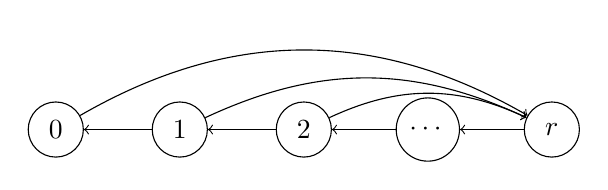
\begin{tikzpicture}[scale=1.05, every node/.style={circle,draw,minimum size=7mm}]
\node (0) at (0,0) {$0$};
\node (1) at (1.5,0) {$1$};
\node (2) at (3.0,0) {$2$};
\node (dots) at (4.5,0) {$\cdots$};
\node (r) at (6.0,0) {$r$};

\draw[->] (0) to[bend left=30] (r);
\draw[->] (1) to[bend left=25] (r);
\draw[->] (2) to[bend left=25] (r);

\draw[->] (2) -- (1);
\draw[->] (1) -- (0);

\draw[->] (r) -- (dots);
\draw[->] (dots) -- (2);

\end{tikzpicture}
\caption{Level transitions for ordinal sums of antichains.}
\label{fig:level_chain}
\end{figure}

\subsection{Top-rank cutoff transfer and metastable slowdown}

Consider a sequence of ordinal sums with fixed $r$ and parameters $(n_1,\dots,n_r)$ and $(p_1,\dots,p_r)$ depending on $N$.
Let $X^{(N)}_t$ be the orbit chain and let $\Pi_{r,N}$ be the stationary mass of the top level $B_r$.
Start the chain from the full ideal $(r,n_r)$.

\begin{theorem}[Top-rank cutoff transfer]\label{thm:top_rank_transfer}
Assume $n_{r,N}\to\infty$, $p_{r,N}\in(0,1)$, and $\Pi_{r,N}\to 1$.
Let
\[
t_N = \frac12\log_{1/p_{r,N}} n_{r,N}.
\]
Then the rowmotion chain started from $(r,n_r)$ exhibits total variation cutoff at time $t_N$ with an $O(1)$ window.
\end{theorem}

\begin{proof}
On the top level $B_r$, the orbit chain restricted to rank $r$ is exactly the Boolean rowmotion chain on an $n_{r,N}$-element antichain with probability $p_{r,N}$, by Proposition~\ref{prop:ordinal_orbit_chain}.
The chain leaves level $r$ only when it is at $(r,n_r)$ and selects all $n_r$ maximal elements, an event of probability $p_{r,N}^{n_{r,N}}$.
Therefore for any $T$,
\[
\PP(\text{leave level }r\text{ by time }T)\le T p_{r,N}^{n_{r,N}}.
\]
With $T=t_N+\cO(1)$ this goes to $0$ because $t_N=\cO(\log n_{r,N})$ while $p_{r,N}^{n_{r,N}}$ decays exponentially.

Let $\pi_{r,N}=\pi_N(\cdot\mid B_r)$.
Conditional on staying in $B_r$ up to time $t$, the law of $X^{(N)}_t$ matches the antichain law on $n_{r,N}$, so by \cite[Theorem 1.6]{DefantLiNestoridi2024Rowmotion} it has cutoff at time $t_N$ with an $O(1)$ window toward $\pi_{r,N}$.
Unconditioning introduces an $o(1)$ error.
Since $\Pi_{r,N}\to 1$, we have $\TV(\pi_{r,N},\pi_N)\to 0$, so cutoff transfers from $\pi_{r,N}$ to $\pi_N$.
\end{proof}

\begin{proposition}[Metastable obstruction when $\Pi_{r,N}$ is not close to $1$]\label{prop:top_rank_obstruction}
Assume $n_{r,N}\to\infty$ and $\limsup_{N\to\infty}\Pi_{r,N}<1$.
Let $t_N=\frac12\log_{1/p_{r,N}} n_{r,N}$.
Then for any fixed $c>0$,
\[
\liminf_{N\to\infty}\ \TV\bigl(\mathcal{L}(X^{(N)}_{\lfloor t_N+c\rfloor}),\pi_N\bigr)
\ge 1-\limsup_{N\to\infty}\Pi_{r,N}.
\]
\end{proposition}

\begin{proof}
The argument in the proof of Theorem~\ref{thm:top_rank_transfer} shows that with probability $1-o(1)$ the chain stays in $B_r$ up to time $\lfloor t_N+c\rfloor$.
On that event the law is close to $\pi_{r,N}$.
Since $\pi_{r,N}$ assigns all mass to $B_r$ and $\pi_N(B_r)=\Pi_{r,N}$,
\[
\TV(\pi_{r,N},\pi_N)=1-\Pi_{r,N}.
\]
The claim follows.
\end{proof}

Proposition~\ref{prop:top_rank_obstruction} shows that when $\Pi_{r,N}$ is not close to $1$, mixing cannot occur on the Boolean cutoff scale $t_N$.
In that regime the explicit inter-level rates in Theorem~\ref{thm:ordinal_exit_rates} indicate an additional, much larger time scale governed by rare transitions between levels.

\section{Discussion}

Rowmotion has long served as a tractable model for global dynamics generated by local combinatorial moves \cite{FonDerFlaass1993,StrikerWilliams2012,ThomasWilliams2019Slow}.
The Markovian randomization of Defant, Li and Nestoridi adds a quantitative mixing layer that interacts strongly with the same local and symmetric structure \cite{DefantLiNestoridi2024Rowmotion}.
The results in this paper suggest that, for many posets, a productive first step in a mixing analysis is a structural reduction that reveals a smaller chain on which the relevant phenomenon is already visible.

A first direction is a structural classification of reductions beyond disjoint unions.
Theorem~\ref{thm:lattice_product_rigidity} shows that lattice products arise only from disconnected posets, but there are many intermediate reductions by strong lumpability.
It would be useful to classify those posets and probability assignments for which the rowmotion chain admits a nontrivial, explicitly describable quotient chain on a state space of polynomial size.

A second direction concerns tensor-power cutoff criteria beyond the Boolean case.
For $P=Q^{\sqcup m}$ we obtained an occupancy lumping with an exact Hellinger isometry, giving a route from one-copy affinity decay to tensor-power cutoff.
General results show that Hellinger and total variation cutoffs coincide under broad hypotheses for product chains \cite{ChenKumagai2018ProductCutoff}.
For many connected $Q$, computing the one-copy affinity $a_x(t)=\BC(\delta_x K^t,\pi)$ remains open and is a natural target for spectral or representation-theoretic methods.

A third direction is to push orbit lumping further into connected symmetric families.
Many posets in dynamical algebraic combinatorics have large automorphism groups, including root posets and related families \cite{Panyushev2009,ArmstrongStumpThomas2013}.
Orbit chains offer a systematic way to translate deterministic orbit phenomena into probabilistic mixing statements, potentially relating homomesy and resonance to concentration of stationary measure and to metastable bottlenecks \cite{ProppRoby2015Homomesy,DilksPechenikStriker2017Resonance}.

A fourth direction is a more complete metastability theory for rowmotion chains.
The complete bipartite orders show a concrete setting where fast within-sector mixing combines with rare between-sector transitions to produce a continuous limiting profile and no cutoff.
For ordinal sums, Proposition~\ref{prop:top_rank_obstruction} shows that nonnegligible stationary mass away from the top rank prevents mixing on the Boolean time scale.
Understanding the longer inter-level equilibration and determining when it yields a continuous profile, and hence no cutoff, is an appealing problem because the orbit chain has fixed level structure but parameter-dependent transition probabilities.

Finally, there are natural model variants.
One can replace the independent Bernoulli choice at each maximal element by other random subset rules, yielding new toggle-type chains on $J(P)$.
One can also consider continuous-time versions, or versions on birational lifts of rowmotion \cite{MusikerRoby2019BirationalPaths}.
Such variants may connect rowmotion mixing questions to integrable probability and to the broader theory of cutoff \cite{Diaconis1996Cutoff}.

\bibliographystyle{elsarticle-num}
\bibliography{refs.bib}

\end{document}
